\documentclass[border=12pt,crop=true]{standalone}
\usepackage{amsmath}
\usepackage{tikz}
\usetikzlibrary{calc, positioning, arrows.meta}

\tikzset{
  tpfig/.style={font=\small},
  tpThin/.style={font=\scriptsize},
  arr/.style={-{Stealth[length=2.2mm]}, thick},
}

% ---------------------------------------------------------------------------
% Layout knobs
% ---------------------------------------------------------------------------
\def\BoxW{3.6}
\def\BoxH{2.0}
\def\PortTop{1.55}
\def\PortBot{0.45}
\def\PortExt{1.35}   % wire length outside box per side
\def\EqGap{0.55}      % gap below box to equation block

\begin{document}
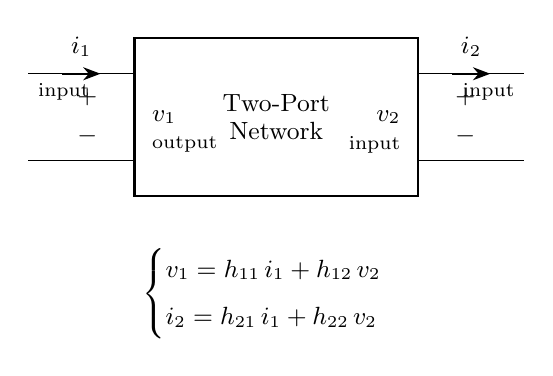
\begin{tikzpicture}[tpfig, >=Stealth]
  % ----- box corners (lower-left origin) -----
  \coordinate (BL) at (0, 0);
  \coordinate (BR) at (\BoxW, 0);
  \coordinate (TL) at (0, \BoxH);
  \coordinate (TR) at (\BoxW, \BoxH);

  % port nodes on box faces
  \coordinate (LT) at (0, \PortTop);
  \coordinate (LB) at (0, \PortBot);
  \coordinate (RT) at (\BoxW, \PortTop);
  \coordinate (RB) at (\BoxW, \PortBot);

  % external terminals
  \coordinate (LextT) at (-\PortExt, \PortTop);
  \coordinate (LextB) at (-\PortExt, \PortBot);
  \coordinate (RextT) at (\BoxW+\PortExt, \PortTop);
  \coordinate (RextB) at (\BoxW+\PortExt, \PortBot);

  % ----- two-port box -----
  \draw[thick] (BL) rectangle (TR);
  \node[align=center] at (\BoxW/2, \BoxH/2)
    {Two-Port\\[-1pt] Network};

  % ----- port 1 (left): i_1 in, v_1 out -----
  \draw (LextT) -- (LT);
  \draw (LextB) -- (LB);
  \draw[arr] ($(LextT)!0.32!(LT)$) -- ($(LextT)!0.68!(LT)$);
  \node[above=1mm] at ($ (LextT)!0.5!(LT) $) {$i_1$};
  \node[tpThin, below right] at (LextT) {input};

  \node[anchor=east] at ($(LT)!0.5!(LB)+(-3.5mm, 2.5mm)$) {$+$};
  \node[anchor=east] at ($(LT)!0.5!(LB)+(-3.5mm, -2.5mm)$) {$-$};
  \node[anchor=west] at ($(LT)!0.5!(LB)+(1mm,0)$) {$v_1$};
  \node[tpThin, anchor=west] at ($(LT)!0.5!(LB)+(1mm,-3.5mm)$) {output};

  % ----- port 2 (right): i_2 in (arrow left into box), v_2 in -----
  \draw (RT) -- (RextT);
  \draw (RB) -- (RextB);
  \draw[arr] ($(RextT)!0.68!(RT)$) -- ($(RextT)!0.32!(RT)$);
  \node[above=1mm] at ($ (RextT)!0.5!(RT) $) {$i_2$};
  \node[tpThin, below left] at (RextT) {input};

  \node[anchor=west] at ($(RT)!0.5!(RB)+(3.5mm, 2.5mm)$) {$+$};
  \node[anchor=west] at ($(RT)!0.5!(RB)+(3.5mm, -2.5mm)$) {$-$};
  \node[anchor=east] at ($(RT)!0.5!(RB)+(-1mm,0)$) {$v_2$};
  \node[tpThin, anchor=east] at ($(RT)!0.5!(RB)+(-1mm,-3.5mm)$) {input};

  % ----- h-parameter equations (centered below box) -----
  \node[anchor=north] at (\BoxW/2, -\EqGap) {%
    $\displaystyle
    \begin{cases}
      v_1 = h_{11}\, i_1 + h_{12}\, v_2 \\[4pt]
      i_2 = h_{21}\, i_1 + h_{22}\, v_2
    \end{cases}$};
\end{tikzpicture}
\end{document}
